\chapter{Patient-Adaptable ECG Classification Framework}

\section{Introduction}
For decades, automatic ECG signal analysis has been a controversial research topic. Several academic research projects have proved that the design and implementation of automatic ECG analysis methods is beneficial for timely detection and therapeutic intervention of heart diseases. However, some major challenges should to be resolved, and automatic ECG analysis should reach a level of maturity and reliability before getting ready for clinical use. One of the most typical challenges is the inherent inter-patient variation of ECG waveforms, which leads to inconsistent performance of ECG classification systems when applied to different patients under different conditions. In this chapter, the details of the patient-adaptable ECG classification method, as the core of the proposed framework are presented.

The goal of automatic ECG analysis is to determine the arrhythmia types for each signal sample. Continuous ECG signal is firstly segmented into individual intervals, each of which represents a heartbeat cycle, to be processed by the further stages of the proposed algorithm. \textcolor{black}{Section 2.2 and Section 2.3} in this chapter focus on the data preparation stage, which includes four steps: signal preprocessing, delineation, segmentation, and feature extraction. Following the data preparation, \textcolor{black}{Section 2.4} elaborates on the details of the proposed two-stage hierarchical classifier. The proposed classification system introduces a novel method for patient-adaptation by gradually capturing the normal range for each individual. More specifically, in Section 2.4, the dynamic normal cluster shaping method to achieve rationalization property is discussed. One feature of this method is that the cluster can track a patient's ECG waveform changes and dynamically adapt to it. In many applications, the physicians need to monitor a long-term real-time heart activity. This dynamic adaptation is able to address the issue of intra-patient temporal signal variation as well.

%In many application scenarios, the method of manual analysis is too complicated and time-consuming to implement. In addition, automatic electrocardiogram analysis has a very important role in monitoring long-term real-time heart activity, because manual monitoring and interpretation are not feasible under these application scenarios. It can be seen that the development of a reliable automatic heartbeat classification algorithm will be conducive to the diagnosis of arrhythmia, so this study will focus on this issue.

%The main goal of this chapter is to introduce the basic framework of automatic heartbeat classification, including ECG signal processing, characterization and classification. The rest of this chapter is organized as follows: Section 2.2 elaborated on the first step of ECG analysis, namely the preprocessing of ECG signals, including filtering and denoising; Section 2.3 immediately follows the previous section, and described the detection methods and periodic segmentation methods for the various peaks in the cardiac cycle. In particular, the multi-stroke segmentation method used in the algorithm described in this article was explained in detail; Section 2.4 introduced the steps of feature extraction and the feature quantities used in this paper based on the segmentation method used in this algorithm. The last section 2.5 is a summary of the contents of this chapter. The author reduced all the steps before the classification algorithm to a mapping and briefly outlined the structure of the classification algorithm.
\section{Utilized Dataset}

Since the quality of ECG signals provided by most of the portable ECG measuring instruments is very unstable and may include transient noises. Signals transmitted through wireless communication systems will exhibit even more unstable waveforms. These transient effects appear in the resulting feature vector and consequently they negatively affect the prediction accuracy of the subsequent ML method. In order to eliminate and smooth out these transient terms, we use the concept of \textit{segmentation} here, where each segment includes multiple cardiac intervals, 
%Moreover, the objective of this work is predictive modeling, thus by including statistical features capturing change between consecutive beats, the system obtains information regarding the following beats. Taking these facts into account, this work performed subsequent feature extraction and analysis combined three consecutive cardiac cycles (i.e. one representative segment). In the subsequent analysis, an segment is considered as a sample of data 
as shown in Fig.~\ref{fig:interval}. \textcolor{blue}{Note that the number of cardiac cycles in each segment is a modeling parameter shown by $s_{window}$. Also, we can arbitrarily slide segments equivalent to $n_{steps}$ cycles to generate the new feature vector. The parameters $s_{window}$ and $n_{steps}$ can be tuned to improve the overall performance of the method.  Based on intensive simulations, we choose $s_{window}=3$ and $n_{steps}=3$, which yield the best classification accuracy. In Fig.~\ref{fig:interval}, we have $s_{window}=3$ and $n_{steps}=1$.}

\begin{figure}[t]
	\centering
	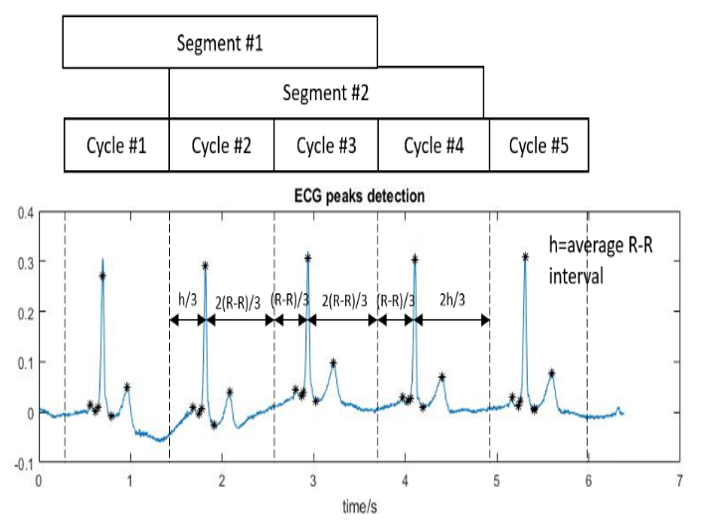
\includegraphics[scale=.8]{Fig/segment.png}
	\caption{Segment samples correspond to three consecutive cardiac cycles.}
	\label{fig:interval}
\end{figure}


%\textcolor{red}{This is not well connected to the text before and after. Make it a separate Section titled as 2.2 Utilized Dataset and move it to the beginning of this section.}
%\subsection{Dataset}
For the purpose of training and evaluating classifier, MITDB is split into test (DS2) and training (DS1) set by balancing the four classes according to \cite{autofs}.


The ECG signals in MITDB dataset are annotated and labels are provided for each cardiac cycle. However, we define a segment, which may include more than one cycle as a sample. Therefore, we need to translate per-cycle labels into per-segment labels. In this regard, a new label for each segment is generated by integrating all annotations of the beats within the segment. The segment is labeled as \textit{normal}, if all member beats are annotated as N; otherwise, this segment will be labeled as the abnormality type of its member cycles if there is only one abnormality type. If more than one abnormality types are present within the same segment, the segment is excluded. \textcolor{black}{For instance, segments with member cardiac cycles labeled "NNN", "SSS", "NVV", "VVV" are respectively mapped to "N","S", "V", and "V", and a segment with member label "NVS" is discarded.} 
After segmentation and new annotation, the total number of samples in the training and test set are obtained as summarized in Table \ref{table:ds}
\begin{table}[t]
	\centering
	\caption{Training and test datasets in MITDB.}
	\vspace{-0.05in}
	\begin{tabular}{|l||c|c|c|c|c|}
		\hline 
		& \multicolumn{4}{c}{Number of segments per AAMI class} &\\ 
		\hline 
		Evaluation Dataset& N & V & S & F &Total \\ 
		\hline 
		DS1:Training & 11721& 2356 & 862 & 256 & 15195\\ 
		\hline 
		DS2:Test & 12633 & 2053 & 550 & 121 & 15357 \\ 
		\hline 
		Total & 24354 & 4409 & 1412 & 377 & 30552 \\ 
		\hline 
	\end{tabular}
	\label{table:ds} 
	\vspace{-0.15in}
\end{table}

\section{ECG Signal Processing}

\subsection{Preprocessing}
Biomedical signals, such as ECG signals,are composed of a sequence of signal segments, that can be presented by a set of statistical, morphological, and spectral features. Since the signal properties change over time, the traditional Fourier transform is not suitable for this type of non-stationary signals since it is unable to capture time-varying statistics of the signal. Wavelet decomposition solves this problem by scaling and translating mother wavelet to constitute its basis functions, which capture both spectral and temporal properties of the signal. Given a time series, wavelet decomposition decomposes the signal into linear combinations of basis functions. Thus, basis functions with larger scales are smoother than those with smaller scales and consequently correspond to lower frequency components of the signal. Similarly, the coefficients of the decomposition correspond to higher frequencies when the scale is smaller. Using wavelet decomposition, we extract both time and frequency features of the signal.

%\textcolor{red}{Here} 

In this work, wavelet analysis is applied to ECG signals in MITDB with a sampling frequency of 360 Hz. Daubechies wavelet of order 8 ($db8$) is selected as mother wavelet for denoising stage in this work for its optimal performance\cite{denoise}. The decomposition coefficients and their corresponding frequency components are presented in Fig. \ref{fig:wavelet_decomp}. %\textcolor{red}{Consistently use Fig. or Figure without dot "." throughout the thesis.}

Low frequency noise or baseline wander between 0.15 to 1 Hz, caused by respiration and body movement, can be removed by deducting the approximation coefficient of level 8 ($A_8$) from the signal. Since the power of ECG signal is mainly concentrated in the frequency band from 1 to 40 Hz, higher frequency terms are more likely to represent noise terms including electromyogram induced noise and mechanical forces acting on the electrodes. These terms can be removed by discarding the detail coefficient of level 1 ($D_1$). 

\subsection{Segmentation}

Most machine learning (ML) algorithms operate on input vectors and are not directly applicable to continuous-signals. Therefore, biomedical signals are typically converted to a representative vector before incorporating to ML algorithms. We follow the common trend of translating a signal segment into a vector of representative features. In this regard, we first need to split the signal in time domain into smaller segments. To obtain more relevant results, we choose the segments as one or multiple consecutive cardiac samples, noting the fact that each cardiac cycles is associated with a label based on experts observation. 

Most existing methods use wavelet analysis to detect the highest peak (R wave) in a cardiac cycle as a reference point and then use signal morphology and typical properties of other waves to determine boundaries between consecutive intervals \textcolor{black}{\cite{banerjee2012delineation,2012qrs,fs,jambukia2015classification}}. In this study, we use this common approach. As was mentioned earlier in Section \ref{sec:fiducial_peaks}, a cardiac cycle consists of five basic characteristic peaks: P, Q, R, S, and T. Among them, the QRS complex is the most significant peak in one cycle. The energy of ECG signal in one cardiac cycle is mainly concentrated within the QRS complex. The QRS complex also conveys important information that reflects the arrhythmia category\cite{2012qrs}. Accurate detection of the QRS complex is of crucial importance for subsequent analysis. The energy of the QRS complex is generally within the range of 5-25 Hz. For ECG signals with sampling frequency of 360Hz, the QRS complex can be extracted from the detail coefficients of level 5 ($D_5$) and level 6 ($D_6$)

\begin{figure}[t]
\centering
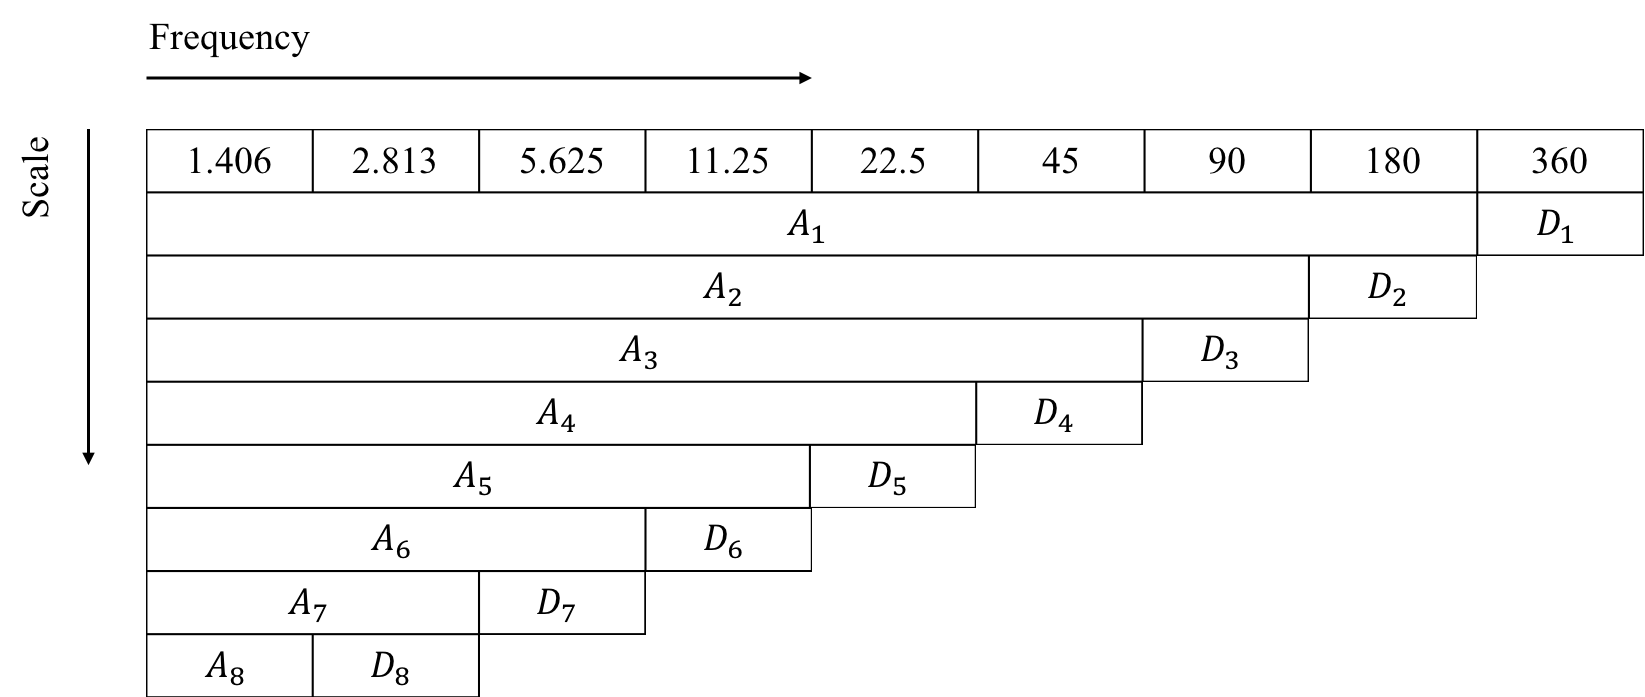
\includegraphics[scale=.5]{Fig/scale_wavelet.png}
\caption{Frequency band of wavelet decomposition coefficients for MITDB signals.}
\label{fig:wavelet_decomp}
\end{figure}


The mother wavelet $db4$ is utilized at this stage due to its morphological similarity to QRS complexes\cite{martinez2004wavelet}. By superimposing $D_5$ and $D_6$, the QRS complex information in the ECG signal can be characterized in a one-dimensional recombined signal ($QRS\_DET = D_5+D_6$).Other Fiducial peaks (P, QRS onset, Q, S, QRS offset and T waves for each cardiac circle) are localized according to an algorithm proposed in \cite{2012qrs}. The accuracy of peak detection and its coincidence with the true signal are shown in Fig. \ref{fig:QRS_d5d6}.

\begin{figure}[t]
\centering
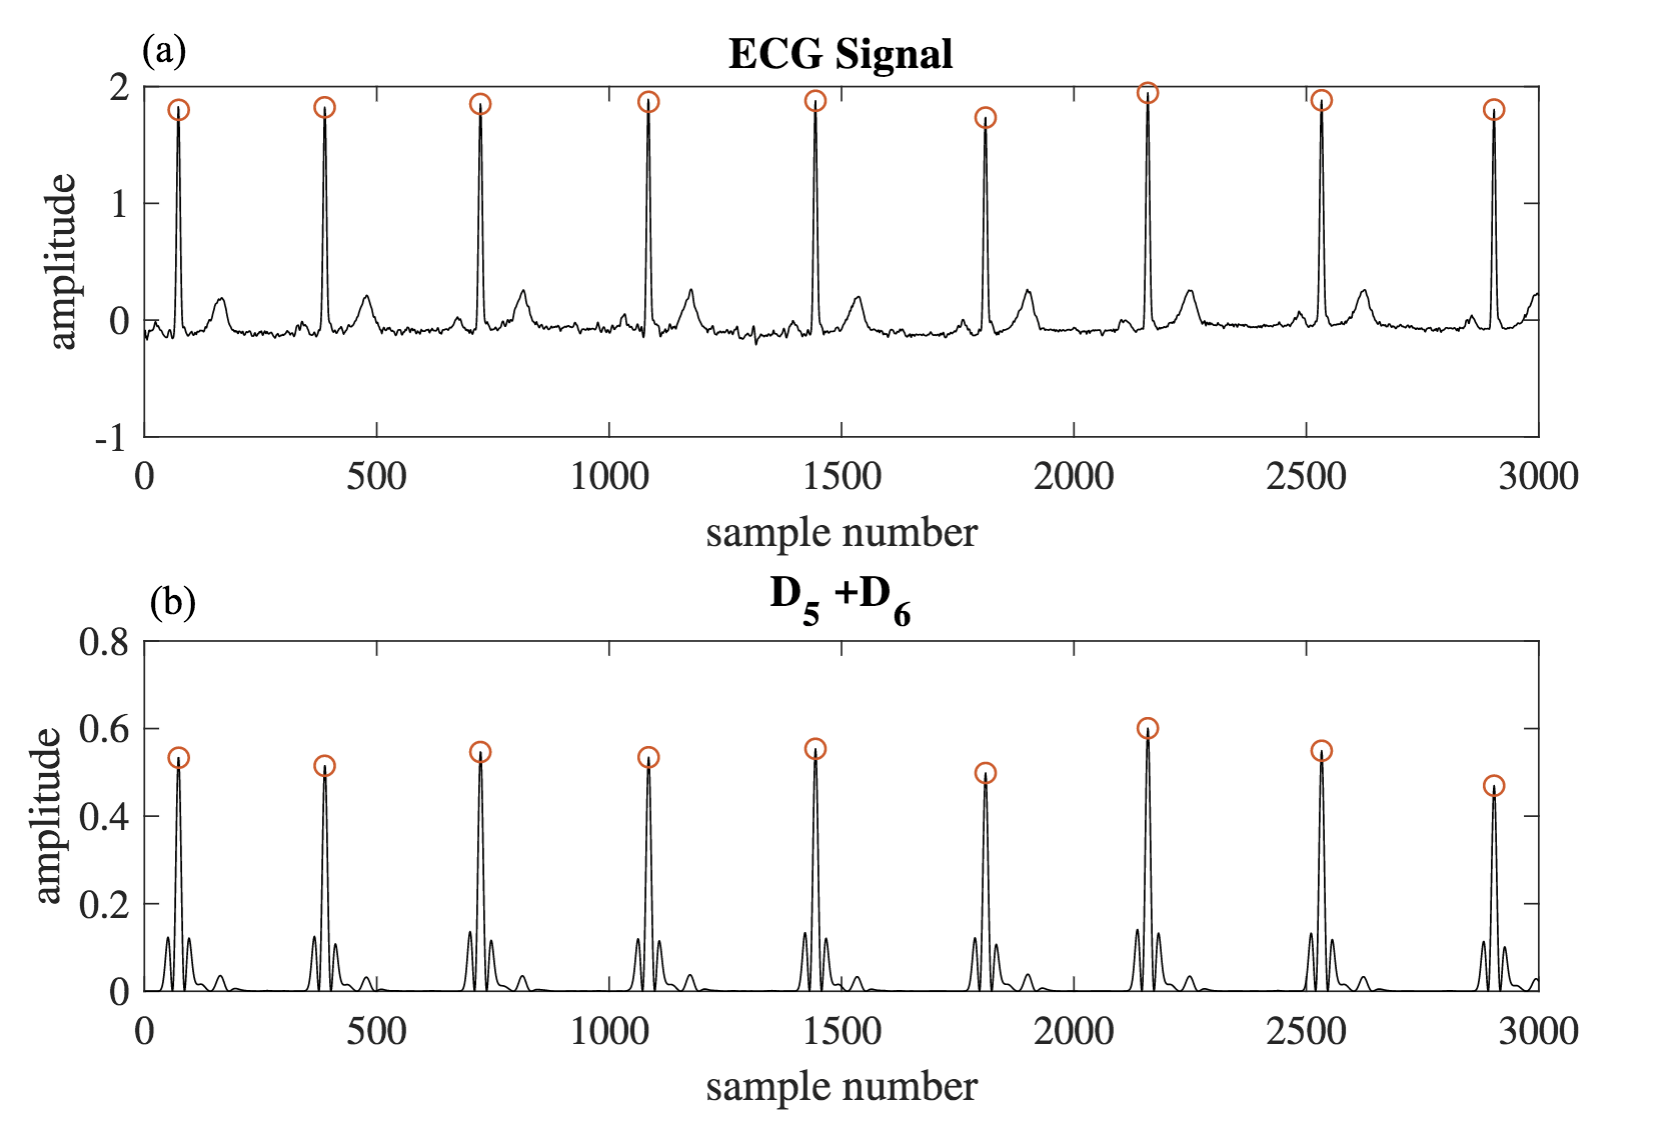
\includegraphics[scale=.5]{Fig/QRS_D5D6_sub.png}
\caption{\textcolor{blue}{(a): the detected R peak location within original ECG signal; (b): corresponding R peak location within the combined signal ($QRS\_DET = D_5+D_6$).} }
	%\textcolor{red}{Add dot to all captions. Also, it is good to use subfigure with captions (a) and (b) and then include the full description in the caption.}}
\label{fig:QRS_d5d6}
\end{figure}


With the empirical values described in \cite{2012qrs}, we use 15\% \textcolor{blue}{of the highest amplitude within the signal} as the detection threshold. Since the width of most of the QRS complexes does not exceed 160ms, here we use a sliding window with a width of 160ms to detect the peaks in the $QRS\_DET$. The window step size is set to 200ms, given that the time lag between the two adjacent heartbeat cycles does not exceed 200ms.  Fig. \ref{fig:window} shows a typical $QRS\_DET$ waveform along with the corresponding window of width 160ms. The false peaks are eliminated using a 160ms time window, as seen in Figure.\ref{fig:window}.


\begin{figure}[t]
\centering
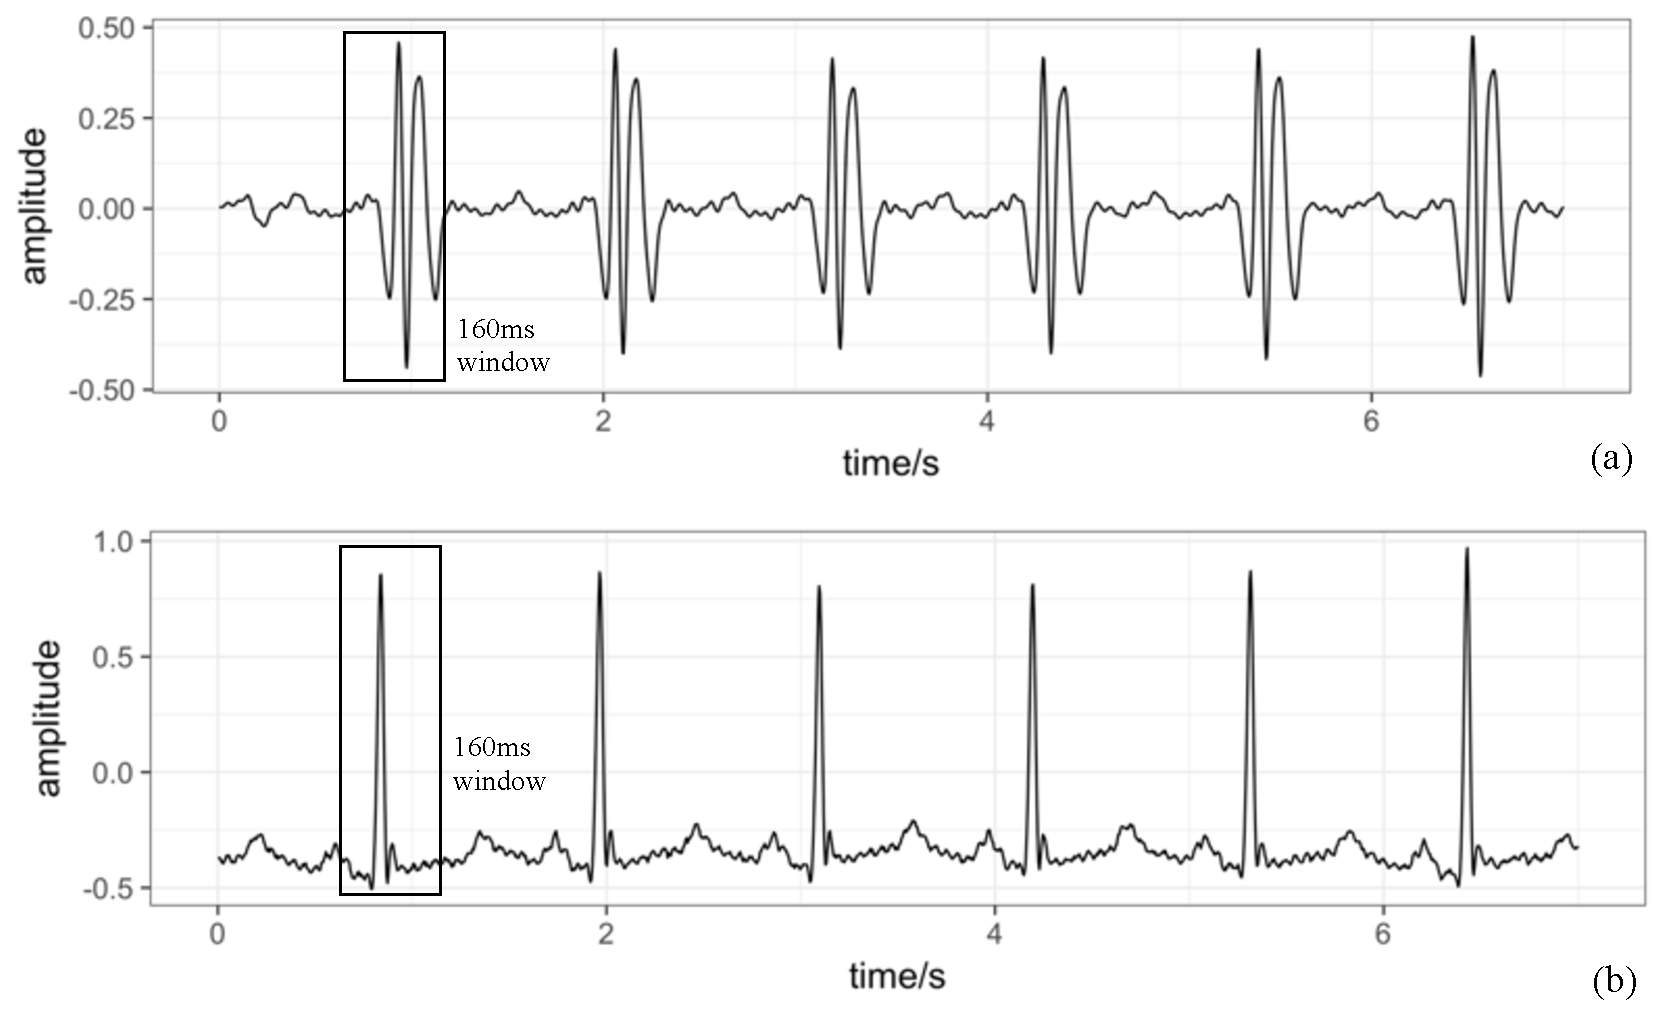
\includegraphics[scale=.5]{Fig/window.pdf}
\caption{Window for detecting R peaks within QRS complexes.}
\label{fig:window}
\end{figure}


The T and P waves are outside the QRS window. Through scanning the region spanning from \textcolor{blue}{the offset of the precedent QRS window to the onset of the current QRS window}%\textcolor{red}{I think you mean: the end of a cardiac interval to the beginning of QRS window in the next interval}
, the P-wave is located as the highest positive peak in this region. In a similar way, the position of the T wave is obtained by finding the maximum of the signal in the region between the offset of the QRS in the current cardiac interval to the onset of the next cardiac interval. \textcolor{black}{In an alternative way, the two peaks between the two consecutive QRS windows, respectively represent the T and P waves.}
In short, an ECG signal in one heartbeat segment can be fully described by 7 feature points: P, QRS on, Q, R, S, QRS off and T. 

After localizing the \textcolor{black}{fiducial peaks}, we can use the location of R peaks to determine the boundaries of a cardiac cycle. %Wwave, a segment of the ECG signal was divided into cardiac cycles. 
By processing a large number of ECG signals, we realize that R peaks approximately split cardiac cycles into two pieces with $1/3$ and $2/3$ of the entire signal\cite{2012qrs}. %\textcolor{red}{Add REF if any}. 
Based on this observation in the morphology of a typical ECG signal, we define the starting point of a cardiac cycle as the point which divides the distance between the two consecutive R waves into two sections, where the length of the first section is half the length of the second section, as depicted in Fig. \ref{fig:interval}. In this figure, the average interval (RR) between the two adjacent R waves is denoted by $h$, therefore R wave is located in distance $h/3$ with respect to the beginning of the cycle. The advantage of this method is its low computational complexity and easy generalization to different patients, noting that a slight change in cardiac boundaries do not significantly alter the properties of a cardiac cycle as long as T and P waves remain in the correct interval. 

%The quality of ECG signals provided by most of the portable ECG measuring instruments is very unstable and may include transient noises. Signals transmitted through wireless communication systems will exhibit even more unstable waveforms. These transient effects appear in the resulting feature vector and consequently they negatively affect the prediction accuracy of the subsequent ML method. In order to eliminate and smooth out these transient terms, we use the concept of \textit{segmentation} here, where each segment includes multiple cardiac intervals, 
%%Moreover, the objective of this work is predictive modeling, thus by including statistical features capturing change between consecutive beats, the system obtains information regarding the following beats. Taking these facts into account, this work performed subsequent feature extraction and analysis combined three consecutive cardiac cycles (i.e. one representative segment). In the subsequent analysis, an segment is considered as a sample of data 
%as shown in Fig.~\ref{fig:interval}. \textcolor{blue}{Note that the number of cycles in each segment is a modeling parameter shown by $XXX$. Also, we can arbitrarily slide segments equivalent to $YYY$ cycles to generate the new feature vector. The parameters $XXX$ and $YYY$ can be tuned to improve the overall performance of the method.  Based on intensive simulations, we choose $XXX=xxx$ and $YYY=yyy$, which yield the best classification accuracy. In Fig.~\ref{fig:interval}, we have $XXX=xxx$ and $YYY=yyy$.}
%
%\begin{figure}[t]
%\centering
%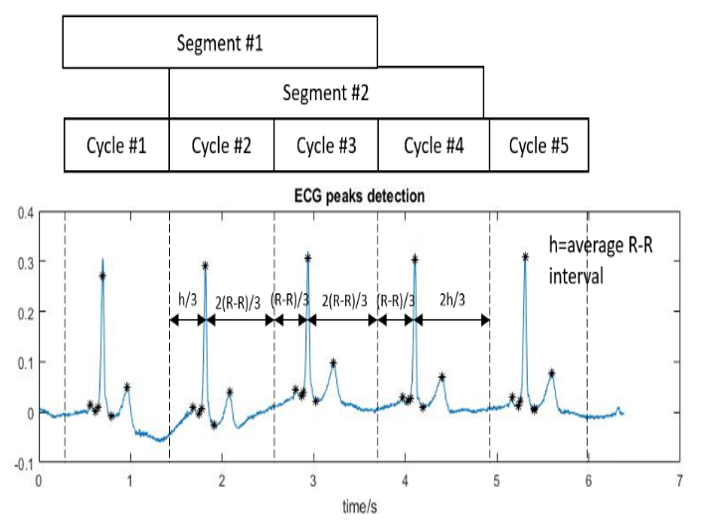
\includegraphics[scale=.8]{Fig/segment.png}
%\caption{Segment samples correspond to three consecutive cardiac cycles}
%\label{fig:interval}
%\end{figure}
%
%
%\textcolor{red}{This is not well connected to the text before and after. Make it a separate Section titled as 2.2 Utilized Dataset and move it to the beginning of this section.}
%%\subsection{Dataset}
%For the purpose of training and evaluating classifier, MITDB is split into test (DS2) and training (DS1) set by balancing the four classes according to \cite{autofs}. 



%The ECG signals in MITDB dataset are annotated and labels are provided for each cycle. However, we define a segment, which may include more than one sample as a sample. Therefore, we need to translate per-cycle labels into per-segment samples. In this regard, a new label for each segment is generated by integrating all annotations of the beats within the segment. The segmend is labeled as \textit{normal}, if all member beats are annotated as N; otherwise, this segment will be labeled as the abnormality type of its member beats if there is only one abnormality type. If more than one abnormality types are present within the same segment, the segment is excluded. \textcolor{blue}{For instance, segments with members labels "NNN", "SSS", "NVV", "VVV" are respectively mapped to "N","S", "V", and "V", and a segment with member label "NVS" is discarded.} 
%After segmentation and new annotation, the total number of samples in the training and test set are obtained as summarized in Table.\ref{table:ds}
%\begin{table}[b]
%	\centering
%	\caption{Training and test datasets in MITDB.}
%	\vspace{-0.05in}
%	\begin{tabular}{|l||c|c|c|c|c|}
%		\hline 
%		& \multicolumn{4}{c}{Number of segments per AAMI class} &\\ 
%		\hline 
%		Evaluation Dataset& N & V & S & F &Total \\ 
%		\hline 
%		DS1:Training & 11721& 2356 & 862 & 256 & 15195\\ 
%		\hline 
%		DS2:Test & 12633 & 2053 & 550 & 121 & 15357 \\ 
%		\hline 
%		Total & 24354 & 4409 & 1412 & 377 & 30552 \\ 
%		\hline 
%	\end{tabular}
%	\label{table:ds} 
%	\vspace{-0.15in}
%\end{table}

\section{Feature Extraction}

The feature extraction step plays a crucial role in the diagnosis of heart disease and has a great influence on the performance of the subsequent automated classification systems. De Chazal et al. have studied the impact of using waveform morphological features on classification results \cite{autofs}. As discussed in \cite{jambukia2015classification}, the combination of three types of characteristics (i.e. temporal, morphology, and frequency domain features) can provide a better discriminative power for the classification algorithm to distinguish between different types of arrhythmia. 

According to several studies different types of ECG signals mainly differ in the power level of the frequency band ranging from 5 Hz to 15 Hz \cite{martinez2004wavelet}. Likewise, some other temporal features (such as the duration between the Q wave and the T wave, the P wave to the R wave, etc.) present different levels of correlation with a specific signal classes \cite{autofs}. Therefore, we choose to use the combination of temporal, morphological and spectral features as detailed in Table \ref{table:features}. Moreover, to account for segment-level characteristics as well as cycle-level properties, the extracted features include both cycle-based features (SET 1) and segment-based features (SET 2). SET1 includes the average and standard deviation of the corresponding features of the three cardiac cycles within a segment, and SET2 contains the overall characteristics of the time signal within a segment, so it is calculated only once per segment. Therefore, we have a total of \textcolor{black}{$8 \times 2 + 6 =22$} features per segment as shown in Table \ref{table:features}. Therefore, each feature vector is a $22×1$ vector with zero-mean unit-variance elements after a proper normalization. %Summarized details are described in Table.\ref{table:features}.
In Table~\ref{table:features}, mean $(R_{i+1}-R_i)$ refers to the mean of the time lag between two adjacent R waves, while $(R_i-R_{avg})$ is the length of each cardiac cycle and the average cardiac cycle duration of the patient. 

\begin{table}[t]
	\caption{Features extracted from ECG signal}%\textcolor{red}{. Change column width such that each line represents one feature.}}
	\label{table:features}
	\centering
	%\begin{flushleft}
	\begin{tabular}{|m{10.5em} | m{11em} |m{11em}|}
		\hline 
		Feature Type & SET1 & SET2 \\ 
		\hline 
		Temporal Features & 
		\tabitem QRS duration & \tabitem  mean$(R_{i+1}-R_i)$ \\
		&\tabitem QT duration &\tabitem mean$(R_i-R_{avg})$ \\
		&\tabitem PR duration & \\
		\hline 
		Morphological Features & \tabitem max positive peak to second peak ratio & \tabitem signal average energy\\
		 & & \tabitem max positive peak \\ 
		 & & \tabitem max negative peak \\ 
		 & & \tabitem peak to energy ratio \\ 
		\hline 
		Frequency Domain Features & \tabitem signal power level at 7.5Hz, 10Hz, 12.5Hz, 15Hz &  \\ 
		\hline 
	\end{tabular} 
	%\end{flushleft}
\end{table}

From Table~\ref{table:features}, one may notice that these 22 features are not completely independent of each other. Also, some of the features may not be as relevant as the others. Therefore, we reduce the number of features to obtain a more robust predictive modeling \cite{autofs, llamedo2012automatic}. We use Principal Component Analysis (PCA) %\textcolor{red}{or principal component analysis (PCA): choose one notation} 
as a commonly used the common dimension reduction method instead of explicit feature selection for its improved performance in biomedical signal processing \cite{castells2007principal}. We keep the 8 dominant directions of the signal after PCA as the most informative 8 features.



\section{Classification Framework}

%\textcolor{red}{part of the following text is related to global classifier, and part of it to deviation analysis (including personalized normal cluster, ...). Use subsections as needed to be more clear.}

In this section, we elaborate on the details of the proposed methodology to perform the classification and prediction tasks using the preprocessed ECG data. Based on our previous study \cite{chen2018predictive} as well as similar prior works on developing patient-specific classifiers \cite{Hu_et_al,deChazal2006,llamedo2012automatic}, we propose a two-staged structure which includes a global classifier to capture general properties of different classes followed by a personalized classifier to capture patient-specific properties~\cite{chen2018predictive,Hu_et_al,deChazal2006,llamedo2012automatic}. Moreover, the proposed algorithm incorporates a novel deviation analysis module with details presented in the following sections. 

\subsection{Global Classifier}

The flowchart in Figure \ref{fig:flow} presents the overall operation of the proposed system. The \textit{global classifier} is trained using the whole training dataset as the first classification step. It facilitates the subsequent analysis in the system by identifying samples with severe morbidity. Depending on the application (properties of signals, the utilized labels, and the choice of features), different classification algorithms can be utilized \cite{Hu_et_al,llamedo2012automatic}. Two important considerations include the classification accuracy and the computation complexity of the method \cite{llamedo2012automatic}. Any abnormal label generated by the global classifier is considered as a \textit{red alarm} and does not require further processing. However, samples labeled as \textit{normal} go through the subsequent personalized classification step. 

\begin{figure}[ht]
	\centering
	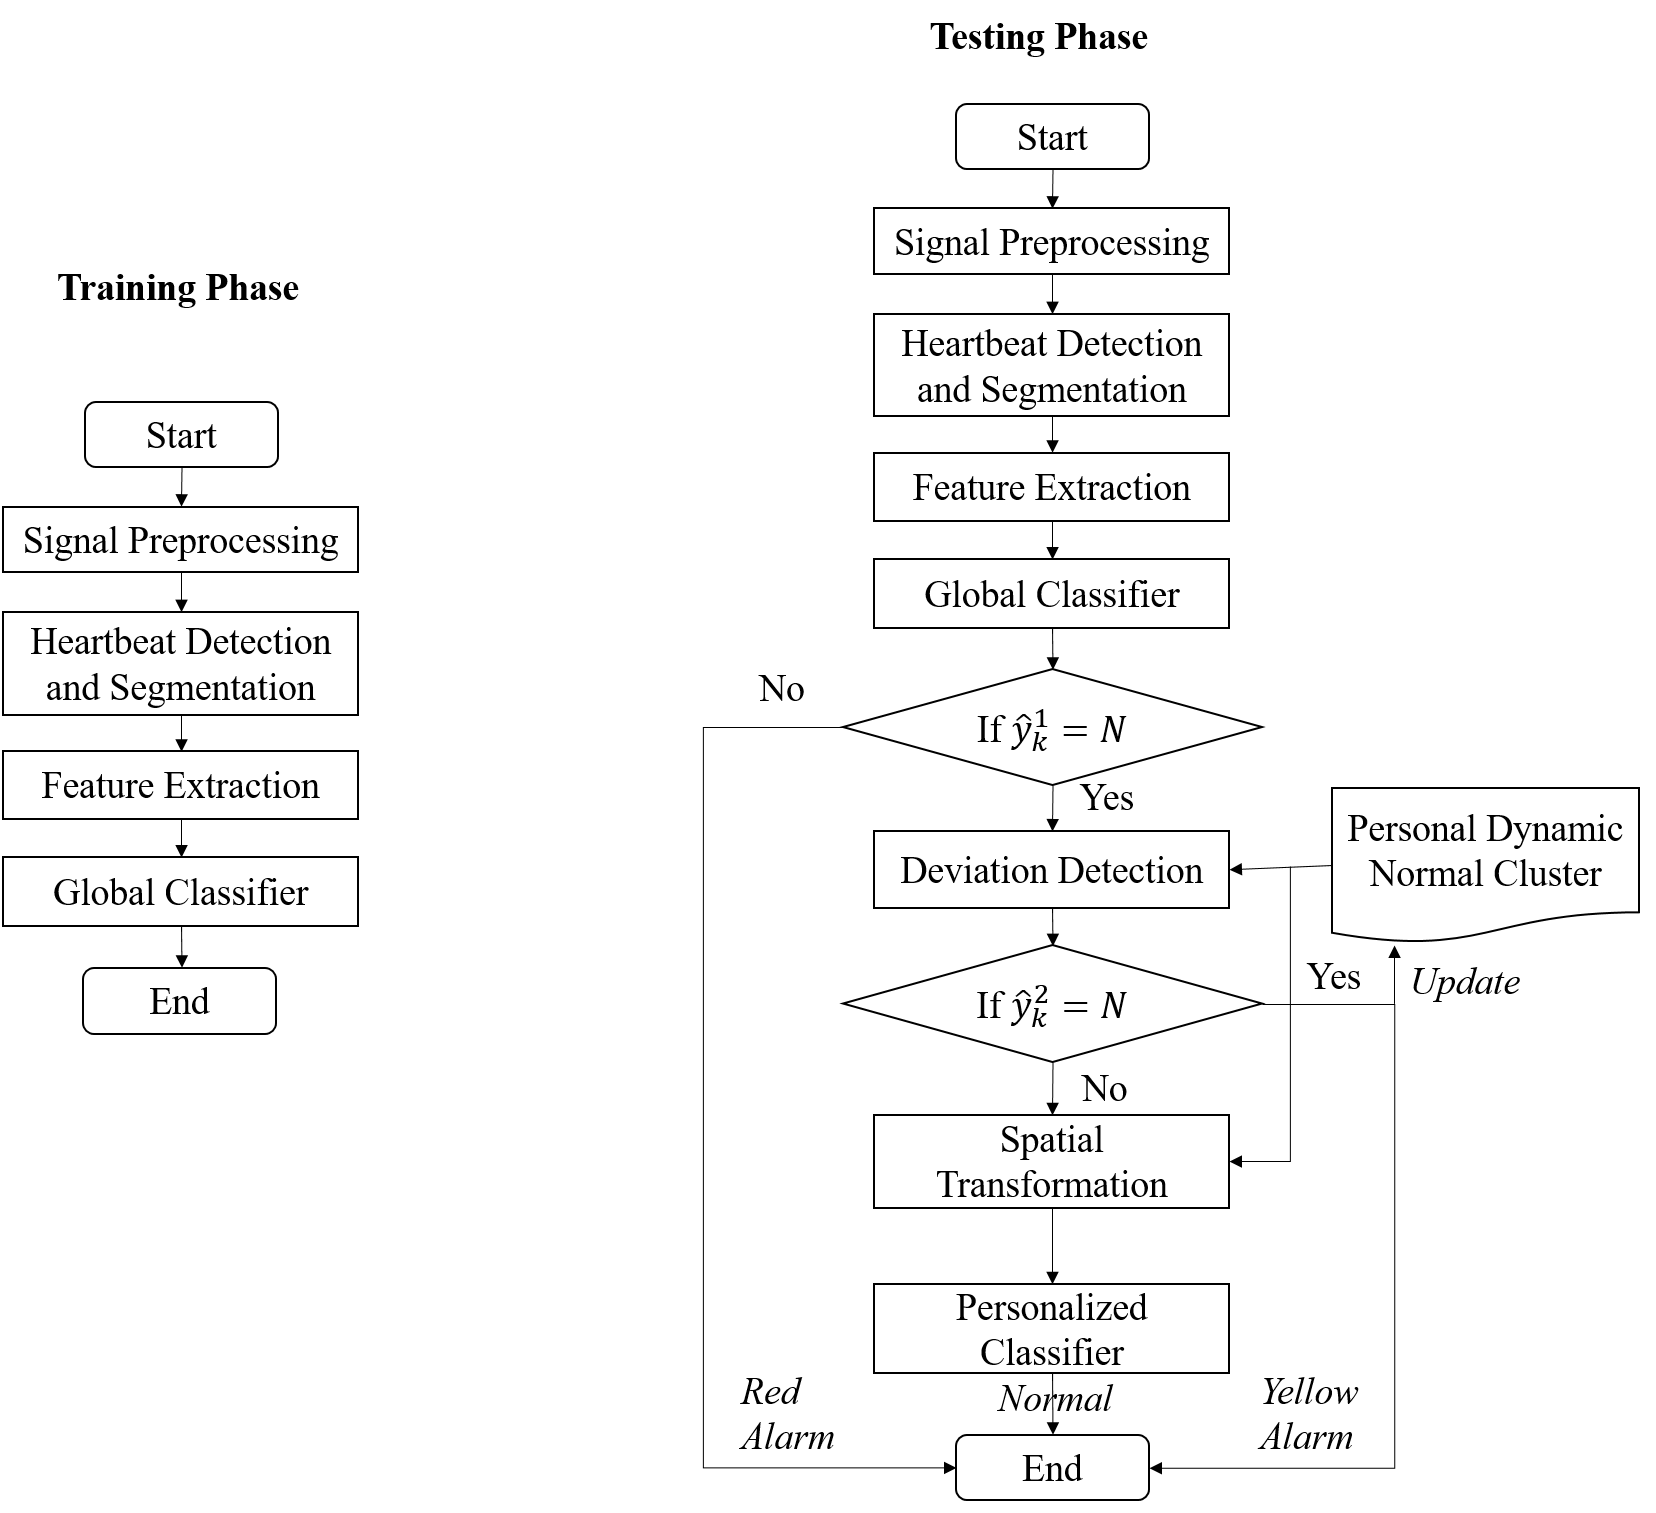
\includegraphics[scale=.5]{Fig/flow2.png}
	\caption{The general flowchart of proposed framework.}
	\label{fig:flow}
\end{figure}


\subsection{Deviation Detection}

Since, one objective of this study is to identify the fuzzy states between normality and abnormalities, the subsequent analysis is focused on processing samples classified as \textit{normal}(N) 
%\textcolor{red}{use a consistent notation: you can choose to use italic font for ``normal'' and ``abnormal'', ``red'', ``yellow'', etc in their first appearance or for all appearances.  Also, define labels N, S, ... on their first appearances.} 
to check whether or not they show considerable deviations towards one of the abnormality classes. For this purpose, a one-layer classifier is not sufficient \textcolor{black}{due to multiple reasons: i) the numbers of samples in the normal and different morbid classes are not balanced in the training set DS1 as shown in Table \ref{table:ds}, ii) the patient-specific normal trend is unknown, iii) detecting yellow alarms require a new set of decision rules to determine whether or not the deviations are worthy of calling a yellow alarm.} Therefore, a deviation detection module is added after the Global Classifier to identify fuzzy state between normality and abnormalities %\textcolor{red}{latent has a special meaning in ML, which is different than what you mean., I recommend change ``latent'' to a different word} %latent status 
using patient-specific normal cluster. In order to develop a ground for patient-specific normal functionality and adapt the classifier accordingly, the first 20\% of total Normal samples of each patient are selected as the initialization of \textit{personalized dynamic normal cluster} $\mathcal{N}_0^k$. \textcolor{blue}{As we collect more samples from the patient, the samples which are newly classified as N class will be used to update the personalized dynamic normal cluster. Therefore, if a sample $\mathbf{x}_k(i)$ is classified as N after deviation detection and the \textit{mahalanobis distance} between $\mathbf{x}_k(i)$ and the centroid of personalized dynamic normal cluster $\mathbf{c}^k_N$ is less than 2, then $\mathbf{x}_k(i)$ is included in the updated $\mathcal{N}_i^k$. mahalanobis distance quantifies how many the standard deviation away $\mathbf{x}_k(i)$ is from $\mathbf{c}^k_N$, it can be formulated as follows:}

\begin{align}
d_{\mathbf{mahal}} = \sqrt{ (\mathbf{x}_k(i)- \mathbf{c}^k_N)' {\rm \bf S}^{-1} (\mathbf{x}_k(i) - \mathbf{c}^k_N) }
\end{align}

where ${\rm \bf S}^{-1}$ stands for the covariance matrix of $\mathcal{N}_i^k$.


To distinguish between normal state and fuzzy state, we use a binary classification of N versus non-N, where the second includes all abnormal classes. We firstly calculate the following distance metrics:

\begin{align}
R_i^{\max}=\underset{\mathbf{x}_j\in\mathcal{N}_i^k,\mathbf{x}_k\in\mathcal{N}_i^k}{\max}\{\sqrt{(\mathbf{x}_j-\mathbf{x}_k)^2}\},\\
\label{eq:matrices}
D_\mathcal{X}(\mathbf{x}_k(i))=\underset{\mathbf{x} \in\mathcal{X}}{\text{median}}\{\sqrt{(\mathbf{x}_k(i)-\mathbf{x})^2}\},
\\
D_\mathcal{N}^{\max}(\mathbf{x}_k(i))=\underset{\mathbf{x} \in\mathcal{N}_i^k}{\text{max}}\{\sqrt{(\mathbf{x}_k(i)-\mathbf{x})^2}\},
%D_V(x^t)=\underset{x_V\in\Omega_V}{\text{median}}\{\sqrt{(x^t-x_V)^2}\}\\
%D_S(x^t)=\underset{x_S\in\Omega_S}{\text{median}}\{\sqrt{(x^t-x_S)^2}\}\\
%D_F(x^t)=\underset{x_N\in\Omega_F}{\text{median}}\{\sqrt{(x^t-x_F)^2}\}\\
%D_{max}(x^t)=\underset{x_N\in\Omega_N^t}{\max}\{\sqrt{(x^t-x_N)^2}\}
\end{align}

The following conditions in Eq. \ref{eq:condition1} are then examined to verify if the deviation of a sample is within the range defined by $\alpha$. Since some rare abnormalities are unlikely to be observed within the limited initialization period, therefore abnormal clusters: ${\mathcal{S},\mathcal{V},\mathcal{F}}$, which include abnormal beats for all patients in DS1, are deployed as the training dataset when \textcolor{blue}{calculating $D_\mathcal{X}(\mathbf{x}_k(i))$ in Eq. \ref{eq:matrices}} %developing the  \textit{personalized dynamic normal cluster} $\mathcal{N}_i^k$ as follows. \textcolor{red}{I think here in $\mathcal{N}_i^k$, you mean that $i=0$ represents the normal cluster and $i=1,2,...$ represent different abnormality clusters. This is not obvious and you need define it before its first appearance.}

\begin{align}\label{eq:condition1}
\begin{cases}
D_\mathcal{N}^{\max}(\mathbf{x}_k(i))  \leq\alpha R_i^{\max},\\
D_\mathcal{N}(\mathbf{x}_k(i)) < D_\mathcal{X}(\mathbf{x}_k(i)) &\text{for~} \mathcal{X}\in\{\mathcal{S},\mathcal{V},\mathcal{F}\}   %(D_N(x^t),D_V(x^t),D_S(x^t),D_F(x^t))=D_N(x^t)
\end{cases}
\end{align}

If a sample already labeled normal by the global classifier, is again confirmed as N in this module, it will be used to update the $\mathcal{N}_i^k$ as mentioned above. Otherwise, the system assumes that the sample has a considerable deviation towards one of the abnormal clusters and hence will pass it to the subsequent \textcolor{black}{\textit{personalized classifier}}. The \textit{personalized classifier} uses controlled transformation with optimized parameters to discern the deviation to different morbid types regardless of the cluster topology within the original feature space\textcolor{black}{, as detailed in Chapters 3 and 4}. 

After performing both global and personalized classification steps, a given sample $x_k(i)$ of patient $i$ at time $k$ is mapped to label $\hat{y}_k \in \{N,Y_V,Y_S,Y_F,R_V,R_S,R_F\}$, where $N$ stands for normal state, $Y_X$ stands for a yellow alarm of type ``X'', and $R_X$ stands for a red alarm of type ``X''.

\begin{figure}[t]
\centering
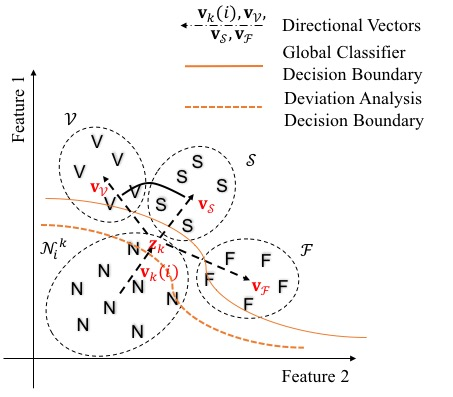
\includegraphics[scale=.7]{Fig/topology.jpg}
\caption{The deviation analysis boundary restrict on latent status between normal and abnormal samples compared with the Global Classifier boundary.}
\label{fig:topo_deviation}
\end{figure}


\section{Personalized Classifier} %\textcolor{red}{I suggest you use the term personalized classifier, although personal classifier is correct too.}

Here, we provide the core idea behind the design of the personalized classifier, and the details of implementation will be discussed in \textcolor{black}{Chapters 3 and 4.} 
Since the proposed system aims at predicting subsequent abnormalities by analyzing a signal's deviation from the patient's normal functionality of the sample signal, it is vital to quantify the deviations using topological characteristics of the training dataset. For most of the ECG applications, ECG signal is analyzed by its representative feature vectors. A natural choice for deviation analysis in the high-dimensional feature space, is \textcolor{black}{\textit{cosine distance}} (as defined in Eq. \ref{eq:cosine}) to quantify the distance between two vectors $\textbf{v}$ and $\textbf{w}$.

\begin{align}
\label{eq:cosine}
d(\mathbf{v},\mathbf{w})= 1 - \frac{\mathbf{v}^T\mathbf{w}}{|\mathbf{v}||\mathbf{w}|}=1 - \frac{\mathbf{v}^T\mathbf{w}}{\sqrt{(\mathbf{v}^T\mathbf{v})(\mathbf{w}^T\mathbf{w})}}
\end{align}

Consequently, relative deviations of a sample from normal cluster(N) to other abnormal clusters (V, S, F) are defined by the cosine distance between the vector $\mathbf{v}_k(i)$ (defined in Eq.\ref{eq:v_k}) and the three vectors $\mathbf{v}_{\mathcal{X}}(i)=\mathbf{c}_{\mathcal{X}}-\mathbf{x}_k(i)$ where $\mathcal{X} \in \{ \mathcal{S}, \mathcal{V}, \mathcal{F}\}$. \textcolor{black}{In this case, a smaller cosine distance represents a higher alignment between the vector from the normal cluster centroid $\mathbf{v}_k(i)$ to the current sample $\mathbf{x}_k(i)$ and the reference vector from the normal cluster centroid to abnormal centroids $\mathbf{c}_{\mathcal{X}}$.}


\begin{align}
\label{eq:v_k}
%\mathbf{v}_k=\mathbf{x}_k-\mathbf{c}_N^k = \mathbf{x}_k- \frac{\sum_{j=1}^{k-1} \mathbf{x}_j I(\hat{y}_j=N)}{\sum_{j=1}^{k-1}  I(\hat{y}_j=N)}, 
\mathbf{v}_k(i)=\mathbf{x}_k(i)-\mathbf{c}_N^k(i) = \mathbf{x}_k(i)- {\sum_{\mathbf{x} \in \mathcal{N}_i^k} \mathbf{x}}/{|\mathcal{N}_i^k|}, 
\end{align}

Therefore, the classification result of the Personal Classifier $\hat{y}^2_k(i)$ is determined as follows:

\begin{align}
\label{eq:personal_discrim}
\hat{y}^2_k(i) = \underset{\mathcal{X} \in \{ \mathcal{S}, \mathcal{V}, \mathcal{F} \}}{\text{argmin}}\{ d(\mathbf{v}_k(i),\mathbf{v}_{\mathcal{X}}(i)) \} 
\end{align}

The relevance of cosine distance depend on the topology of clusters in the feature space. The topology in feature space, itself is inherited from the feature extraction and feature selection methods. For example, as shown in Fig.\ref{fig:topo1}, in the original feature space overlaps and alignment of abnormal clusters may lead to inaccurate results of deviation quantification. \textcolor{black}{In order to eliminate the deviation analysis errors that arise from the asymmetry in the topology of clusters, it is desired to transform the original topology into a more symmetric one, where cosine distances directly reflect the amount of deviations.}

\begin{figure}[thpb]
\centering
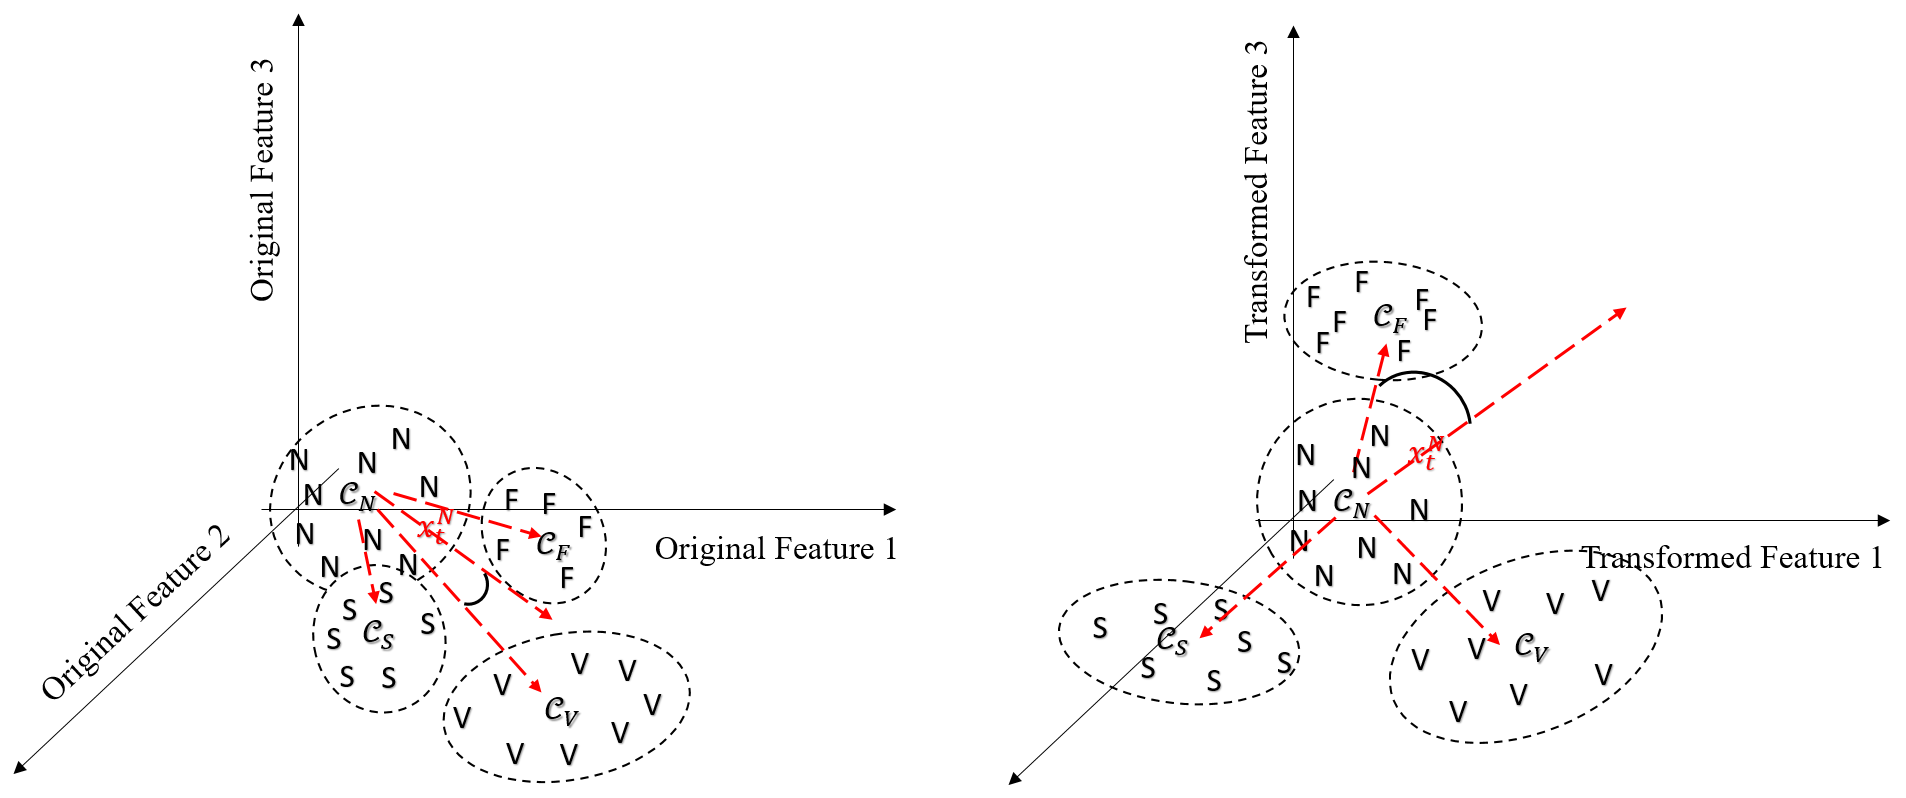
\includegraphics[scale=.5]{Fig/topo1.png}
\caption{Left: illustration of the cluster topology in the original feature space; Right: illustration of the cluster topology in the transformed feature space using a nonlinear mapping function.}
\label{fig:topo1}
\end{figure}

For this purpose, two different spatial transformation methods are proposed in the next two chapters.

